% tikz_levels.tex -- the density bound of sec:density-cells.
%   (a) For each count M of centres within sqrt6 from 24 to 30, the proved upper bound for the
%       union of caps U(Y) (prop:levels), against the level 9pi^2/8 - 8 that statement (C) asks
%       for and the level below which the density bound would pass the three-point bound.
%   (b) The resulting density bound on a scale with the other bounds for R^4.
% Data: the unconditional bounds printed by radial_case_check.py for the certificates
%       multi_cap/radial_certificates/density_M.json (M = 25..30), and 24 S(2) for M = 24.
% Build:  pdflatex tikz_levels.tex && pdftoppm -r 500 -png -singlefile tikz_levels.pdf ../figures/fig_tikz_levels
% Test:   python3 tikz_overlap_check.py tikz_levels.tex
\documentclass[border=4pt]{standalone}
\usepackage{tikz}
\usepackage{pgfplots}
\pgfplotsset{compat=1.17}
\usetikzlibrary{positioning,arrows.meta,calc}
\usepackage[T1]{fontenc}
\usepackage{lmodern}
\usepackage{amsmath,amssymb}
\definecolor{cblue}{HTML}{2A78D6}
\definecolor{corange}{HTML}{EB6834}
\definecolor{caqua}{HTML}{1BAF7A}
\definecolor{cviolet}{HTML}{4A3AA7}
\definecolor{cink2}{HTML}{52514E}
\definecolor{cink3}{HTML}{8B8A85}
\def\Lsix{3.3524}
\def\Dsix{0.63668}
% tikzcheck.tex -- the hooks of tikz_overlap_check.py, input by the TikZ figures.
% Two ways to name what is checked.
%  - Explicit: \figboxes and \figlabels list named nodes; with \nolabels defined,
%    nodes in the style lbl are drawn invisibly.
%  - Automatic: \autocheck in the preamble gives every node of the picture,
%    pgfplots tick labels included, an alias chk<n>; with \nolabels defined, the
%    text of every node is drawn invisibly and its shape is kept.
% \checkfigure, at the end of the picture, writes the four corners of each
% checked node (so that rotated nodes are measured by their true extent) and
% those of the picture to the log when \checkbboxes is defined.
\tikzset{lbl/.style={}}
\ifdefined\nolabels\tikzset{lbl/.append style={opacity=0}}\fi
\newcount\chknodes
\newcommand\autocheck{% idempotent: a figure with \autocheck may also be run with --auto
  \ifdefined\chkauto\else
  \def\chkauto{}%
  \tikzset{every node/.append style={/utils/exec={\global\advance\chknodes by 1\relax},
                                      alias=chk\the\chknodes}}%
  \ifdefined\nolabels\tikzset{every node/.append style={text opacity=0}}\fi
  \fi}
\makeatletter
% a node counted but never kept (pgfplots typesets some nodes once to measure them)
% has no shape, and is skipped
\newcommand\chkifnode[2]{\pgfutil@ifundefined{pgf@sh@ns@#1}{}{#2}}
\makeatother
\newcommand\chkout[2]{% kind, node
  \path let \p1=(#2.south west), \p2=(#2.north east), \p3=(#2.north west), \p4=(#2.south east)
    in \pgfextra{\typeout{BBOX #1 #2\space\x1\space\y1\space\x2\space\y2\space\x3\space\y3\space\x4\space\y4}};}
\newcommand\checkfigure{%
  \ifdefined\checkbboxes
    \path let \p1=(current bounding box.south west), \p2=(current bounding box.north east)
      in \pgfextra{\typeout{PICBB \x1\space\y1\space\x2\space\y2}};
    \typeout{BORDER 4.0pt}%
    \ifdefined\chkauto
      \edef\chklast{\the\chknodes}%
      \foreach \nm in {1,...,\chklast} {\chkifnode{chk\nm}{\chkout{auto}{chk\nm}}}%
    \else
      \foreach \nm in \figboxes {\chkout{box}{\nm}}%
      \foreach \nm in \figlabels {\chkout{label}{\nm}}%
    \fi
  \fi}
\ifdefined\forceauto\autocheck\fi

\begin{document}
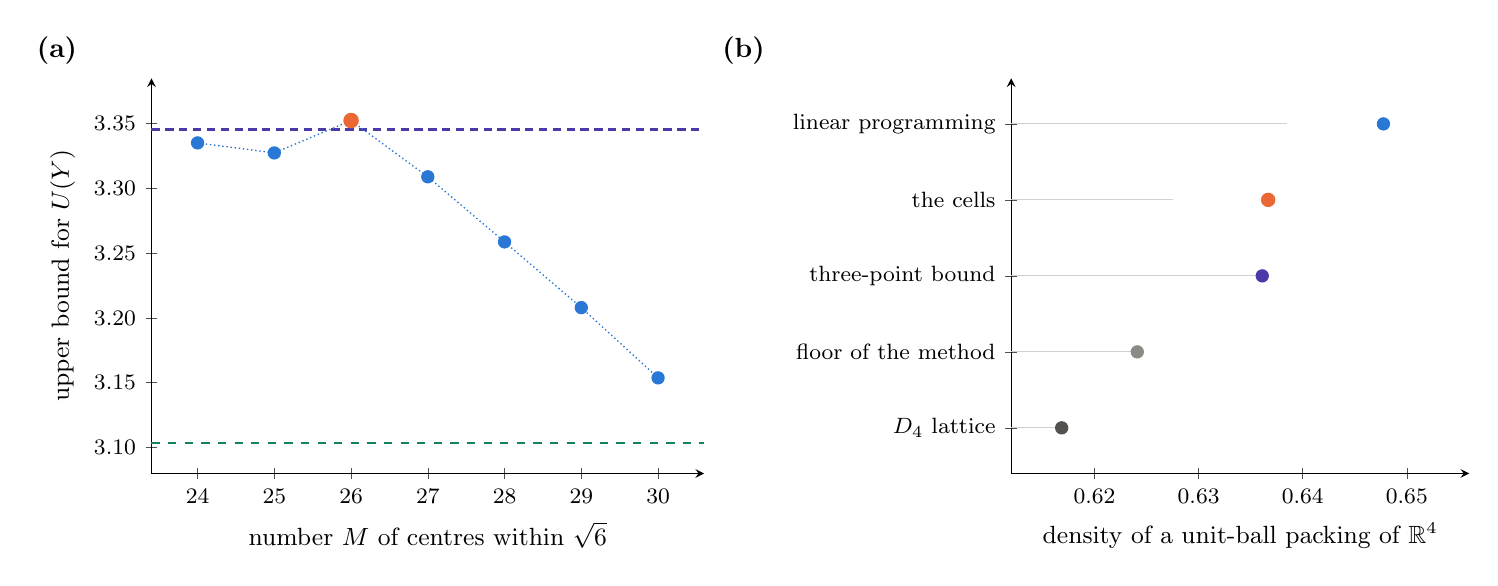
\begin{tikzpicture}[font=\small]
\begin{axis}[name=A, width=8.6cm, height=6.6cm,
    xmin=23.4, xmax=30.6, ymin=3.08, ymax=3.385,
    xtick={24,...,30}, ytick={3.1,3.15,3.2,3.25,3.3,3.35},
    yticklabels={$3.10$,$3.15$,$3.20$,$3.25$,$3.30$,$3.35$},
    xlabel={number $M$ of centres within $\sqrt6$}, ylabel={upper bound for $U(Y)$},
    axis lines=left, tick style={cink2}, tick label style={font=\footnotesize},
    scaled y ticks=false, clip=false]
  \draw[caqua!75!black, line width=0.8pt, dashed] (axis cs:23.4,3.10330) -- (axis cs:30.6,3.10330);
  \draw[cviolet, line width=0.8pt, densely dashed] (axis cs:23.4,3.34549) -- (axis cs:30.6,3.34549);
  \addplot[cblue, line width=0.5pt, densely dotted, mark=none] coordinates
    {(24,3.33513) (25,3.32739) (26,\Lsix) (27,3.30896) (28,3.25870) (29,3.20799) (30,3.15376)};
  \addplot[only marks, mark=*, mark size=2.2pt, cblue] coordinates
    {(24,3.33513) (25,3.32739) (27,3.30896) (28,3.25870) (29,3.20799) (30,3.15376)};
  \addplot[only marks, mark=*, mark size=2.6pt, corange] coordinates {(26,\Lsix)};
  \coordinate (A-c) at (axis cs:30.6,3.10330);
  \coordinate (A-r) at (axis cs:26.75,3.3505);
  \coordinate (A-26) at (axis cs:26,\Lsix);
  \coordinate (A-24) at (axis cs:24,3.33513);
  \coordinate (A-25) at (axis cs:25,3.32739);
  \coordinate (A-27) at (axis cs:27,3.30896);
  \coordinate (A-28) at (axis cs:28,3.25870);
  \coordinate (A-29) at (axis cs:29,3.20799);
  \coordinate (A-30) at (axis cs:30,3.15376);
\end{axis}
\node[lbl, inner sep=1pt, font=\footnotesize, anchor=west, text=caqua!65!black, align=left] (lc) at ($(A-c)+(0.1,0)$)
  {$9\pi^2/8-8$:\\statement (C)};
\node[lbl, inner sep=1pt, font=\footnotesize, anchor=south west, text=cviolet] (lr) at (A-r)
  {$3.34549$: the three-point bound};
\node[lbl, inner sep=1pt, font=\footnotesize, anchor=south, yshift=3pt, text=corange!85!black] (l26) at (A-26) {$\Lsix$};
\node[lbl, inner sep=1pt, font=\scriptsize, anchor=north, yshift=-4pt, text=cblue!85!black] (l24) at (A-24) {$3.3352$};
\node[lbl, inner sep=1pt, font=\scriptsize, anchor=north, yshift=-4pt, text=cblue!85!black] (l25) at (A-25) {$3.3274$};
\node[lbl, inner sep=1pt, font=\scriptsize, anchor=south west, xshift=2pt, yshift=2pt, text=cblue!85!black] (l27) at (A-27) {$3.3090$};
\node[lbl, inner sep=1pt, font=\scriptsize, anchor=south west, xshift=2pt, yshift=2pt, text=cblue!85!black] (l28) at (A-28) {$3.2587$};
\node[lbl, inner sep=1pt, font=\scriptsize, anchor=south west, xshift=2pt, yshift=2pt, text=cblue!85!black] (l29) at (A-29) {$3.2080$};
\node[lbl, inner sep=1pt, font=\scriptsize, anchor=south west, xshift=2pt, yshift=2pt, text=cblue!85!black] (l30) at (A-30) {$3.1538$};
\begin{axis}[name=B, at={($(A.east)+(3.9cm,0)$)}, anchor=west, width=7.4cm, height=6.6cm,
    xmin=0.612, xmax=0.656, ymin=0.4, ymax=5.6,
    ytick={1,2,3,4,5}, yticklabels={$D_4$ lattice, floor of the method, three-point bound, the cells, linear programming},
    xtick={0.62,0.63,0.64,0.65}, xticklabels={$0.62$,$0.63$,$0.64$,$0.65$},
    xlabel={density of a unit-ball packing of $\mathbb{R}^4$},
    axis lines=left, tick style={cink2}, tick label style={font=\footnotesize},
    scaled x ticks=false, clip=false]
  \draw[cink3!40, line width=0.4pt] (axis cs:0.612,1) -- (axis cs:0.6162,1);
  \draw[cink3!40, line width=0.4pt] (axis cs:0.612,2) -- (axis cs:0.6235,2);
  \draw[cink3!40, line width=0.4pt] (axis cs:0.612,3) -- (axis cs:0.6355,3);
  \draw[cink3!40, line width=0.4pt] (axis cs:0.612,4) -- (axis cs:0.6275,4);
  \draw[cink3!40, line width=0.4pt] (axis cs:0.612,5) -- (axis cs:0.6385,5);
  \addplot[only marks, mark=*, mark size=2.2pt, cink2] coordinates {(0.61685,1)};
  \addplot[only marks, mark=*, mark size=2.2pt, cink3] coordinates {(0.62411,2)};
  \addplot[only marks, mark=*, mark size=2.2pt, cviolet] coordinates {(0.63611,3)};
  \addplot[only marks, mark=*, mark size=2.4pt, corange] coordinates {(\Dsix,4)};
  \addplot[only marks, mark=*, mark size=2.2pt, cblue] coordinates {(0.64775,5)};
  \coordinate (B-1) at (axis cs:0.61685,1);
  \coordinate (B-2) at (axis cs:0.62411,2);
  \coordinate (B-3) at (axis cs:0.63611,3);
  \coordinate (B-4) at (axis cs:\Dsix,4);
  \coordinate (B-5) at (axis cs:0.64775,5);
\end{axis}
\node[lbl, inner sep=1pt, font=\footnotesize, anchor=west, xshift=3pt, text=cink2] (lb1) at (B-1) {$0.61685$};
\node[lbl, inner sep=1pt, font=\footnotesize, anchor=west, xshift=3pt, text=cink3] (lb2) at (B-2) {$0.62411$};
\node[lbl, inner sep=1pt, font=\footnotesize, anchor=west, xshift=3pt, text=cviolet] (lb3) at (B-3) {$0.63611$};
\node[lbl, inner sep=1pt, font=\footnotesize, anchor=east, xshift=-3pt, text=corange!85!black] (lb4) at (B-4) {$\Dsix$};
\node[lbl, inner sep=1pt, font=\footnotesize, anchor=east, xshift=-3pt, text=cblue!85!black] (lb5) at (B-5) {$0.64775$};
\node[font=\bfseries] (pa) at ($(A.north west)+(-1.2cm,0.35cm)$) {(a)};
\node[font=\bfseries] (pb) at ($(B.north west)+(-3.4cm,0.35cm)$) {(b)};
\def\figboxes{pa,pb}
\def\figlabels{lc,lr,l26,l24,l25,l27,l28,l29,l30,lb1,lb2,lb3,lb4,lb5}
\checkfigure
\end{tikzpicture}
\end{document}
